\begin{theorem}[Сидлер]
    Пусть для двух равновеликих многогранников все инварианты Дена равны, то есть для любой аддитивной функции, определённой на их двугранных углах и числе $\pi$, выполнено $f(\pi) = 0, \ f(W_1) = f(W_2) \Rightarrow W_1, W_2$ равносоставлены.
\end{theorem}
\begin{proof}
    Кажется, было без доказательства.
\end{proof} 

\subsection{Третья проблема Гильберта}
\begin{definition}
    Два равновеликих многогранника $A, B$ называются \textit{равнодополняемыми}, если существуют два равносоставленных многогранника $W_A, W_B$, для которых существуют разбиения $W_A = \bigcup_{i = 1}^k P_i \cup A, \ W_B = \bigcup P_i \cup B$, где $P_i$ — многогранники.
\end{definition}

\noindent \textbf{3-я проблема Гильберта.}
\textit{Существуют ли не равнодополняемые тетраэдры с равными основаниями и высотами?}

\begin{statement}
    Если многогранники $A,B$ равнодополняемые, то их инварианты Дена равны.
\end{statement}
\begin{proof}
    $f(W_A) = f(W_B)$, где $$f(W_A) = f(A) + \sum_{i = 1}^{k} f(P_i) = f(B) + \sum_{i = 1}^{k} f(P_i) = f(W_B)$$
\end{proof}

\begin{definition}
    Координатный тетраэдр — тетраэдр с вершинами с координатами $(0,0,0), (1,0,0), (0,1,0), (0,0,1)$ или подобный ему.
\end{definition} 

\begin{figure}[htbp]
    \centering
    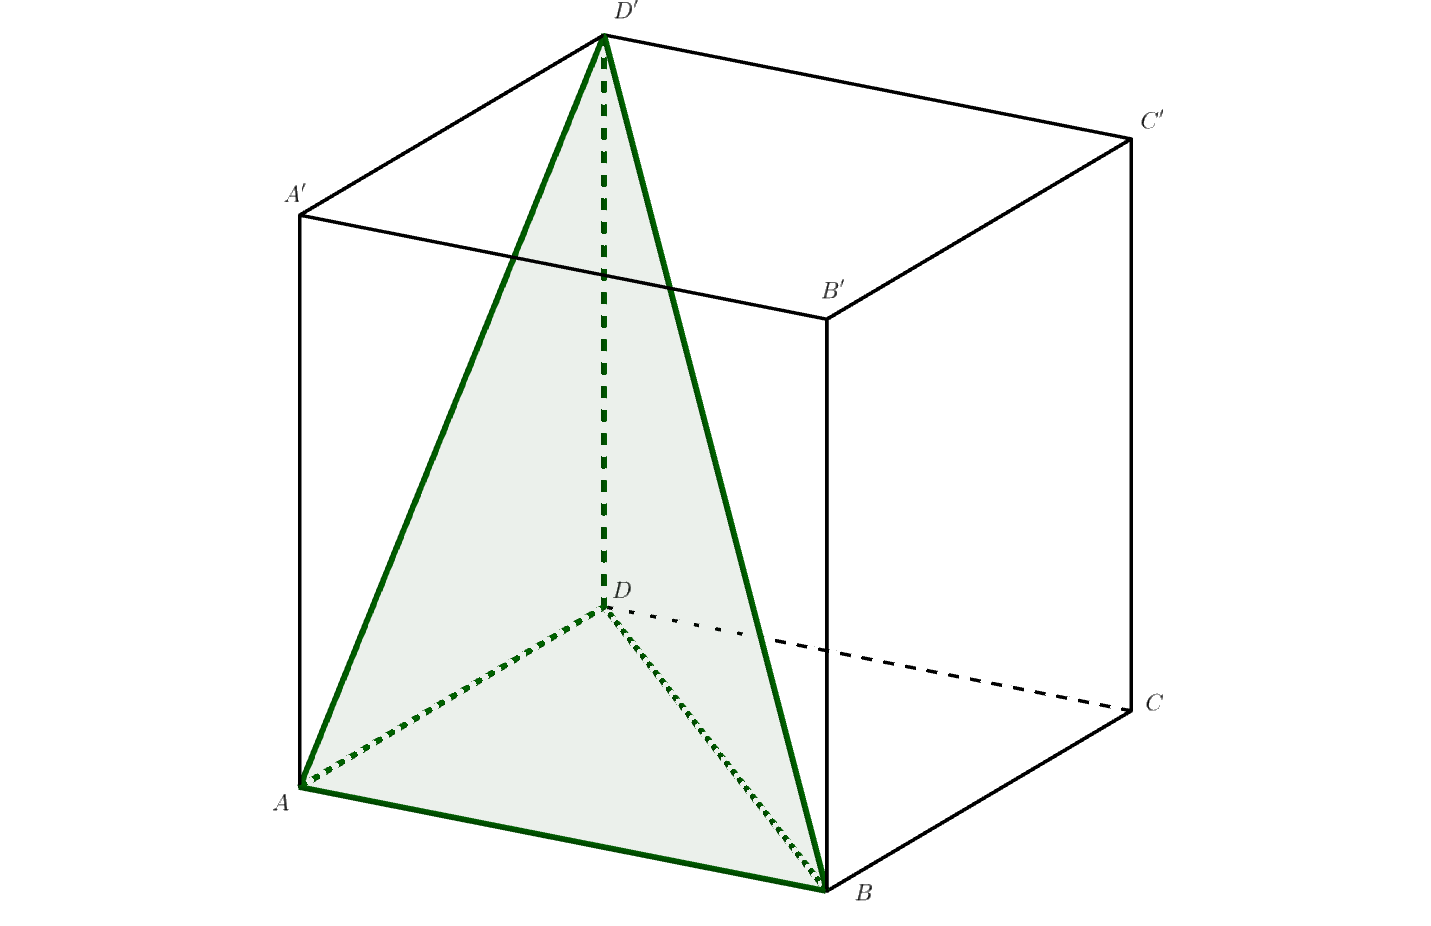
\includegraphics[scale=0.2]{images/c9.7.png}
    \caption{Тетраэдр Хилла.}
    \label{fig:c9.7}
\end{figure}

\begin{definition}
    Тетраэдр Хилла — тетраэдр, у которого основание — равнобедренный прямоугольный треугольник, высота равна катету основания и падает в один из концов гипотенузы основания.
\end{definition} 
% Сюда тетраэдр Хилла.
\begin{figure}[htbp]
    \centering
    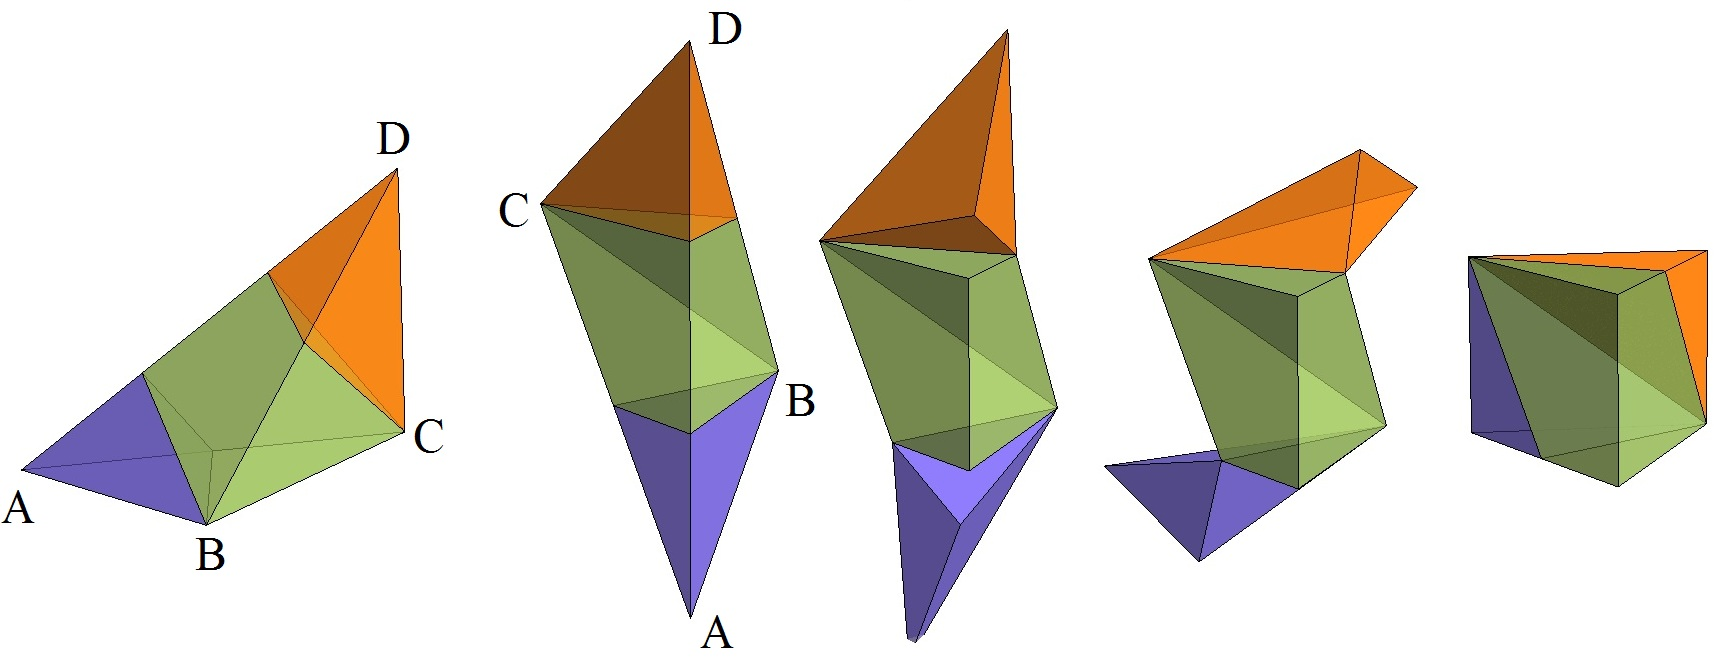
\includegraphics[scale=0.2]{images/c9.8.png}
    \caption{Тетраэдр Хилла равносоставлен с прямоугольной призмой}
    \label{fig:c9.8}
\end{figure}

\begin{statement}
    Тетраэдр Хилла равносоставлен с прямоугольной призмой.
\end{statement} 
\begin{proof}
    См.рис.\ref{fig:c9.8}.
\end{proof} 

\begin{statement}
    Каждый инвариант Дена тетраэдра Хилла равен нулю.
\end{statement} 
\begin{proof}
    Данное утверждение — следствие утверждения, которое было только что, и теоремы о равнодополняемых многогранниках.

    У тетраэдра Хилла каждый инвариант Дена такой же, как и у призмы. Так как каждый инвариант Дена для призмы равен нулю, то и для тетраэдра Хилла он также равен нулю.
\end{proof} 

\begin{statement}
    У координатного тетраэдра имеется ненулевой инвариант Дена.
\end{statement} 
\begin{proof}
    Обозначим через $\alpha$ величину двугранного угла при рёбрах грани, являющейся правильным треугольником. Тогда $\cos{\alpha} = 1 / \sqrt{3}$. Число $\frac{1}{\pi} \arccos{1/\sqrt{3}}$ иррационально. Отсюда следует, что множество $\{\alpha, \pi/2, \pi\}$ не имеет зависимостей, в которые $\alpha$ входит с ненулевым коэффициентом.

    Поэтому, положив $f(\alpha) = 1, \ f(\pi/2) = 0, \ f(\pi) = 0$, получим функцию Дена для координатного тетраэдра. Соответствующий ей инвариант Дена не равен нулю.
\end{proof} 

\begin{statement}[Решение третьей проблемы Гильберта]
    Тетраэдр Хилла и координатный тетраэдр не равносоставлены, а также не равнодополняемы.
\end{statement}
\begin{proof}
    Пусть $f$ — функция Дена, построенная в доказательстве выше. Тогда её значения на координатном тетраэдре отлично от нуля. Продолжим $f$ до функции Дена для тетраэдра Хилла. Однако любой инвариант Дена для тетраэдра Хилла равен нулю. Следовательно, тетраэдр Хилла и координатный тетраэдр не являются равнодополняемыми.
\end{proof} 

\newpage
\section{Многообразия}

\begin{definition}
    Пусть $X$ — топологическое пространство. Пусть $B$ — семейство его открытых подмножеств такое, что любое открытое множество в $X$ есть объединение множеств из $B$. $B$ называется \textit{базой топологии}.
\end{definition}

\begin{definition}
    Хаусдорфово топологическое пространство называется \textit{двумерным ($n$-мерным) многообразием}, если оно имеет счётную базу, и у любой точки существует окрестность, гомеоморфная открытому двумерному ($n$-мерному) диску.
\end{definition}

\begin{remark}
    По сути, мы задали определение $n$-мерного многообразия \textit{без края}. $n$-мерное многообразие \textit{с краем} — это хаусдорфово топологическое пространство со счётной базой, в котором каждая точка имеет окрестность, гомеоморфную открытому подмножеству замкнутого полупространства в $\R^n$ (полукругу, то есть).
\end{remark}

\begin{remark}
    Точки, которые имеют открытую окрестность, гомеоморфную открытому двумерному диску, будем называть \textit{внутренними}, а множество всех таких точек — \textit{внутренностью многообразия}.
\end{remark}

\subsection{Классификация двумерных связных компактных многообразий}

Примеры:
\begin{enumerate}
    \item $\R^2$ — плоскость — не компактна, без края;
    \item Сфера — компактна, без края;
    \item Тор (см.рис.\ref{fig:thorus}) — компактен, без края;
    \item Бутылка Клейна (см.рис.\ref{fig:kleyn}) — компактна, без края;
    \item Проективная плоскость $\R P^2$ — компактна, без края;
    \item Диск — компактен, с краем;
    \item Цилиндр без крышки — компактен, с краем;
    \item Лист Мёбиуса (см.рис.\ref{fig:mobius}) — с краем;
\end{enumerate}

\begin{figure}[htbp]
    \centering
    \begin{subfigure}[b]{0.48\textwidth}
        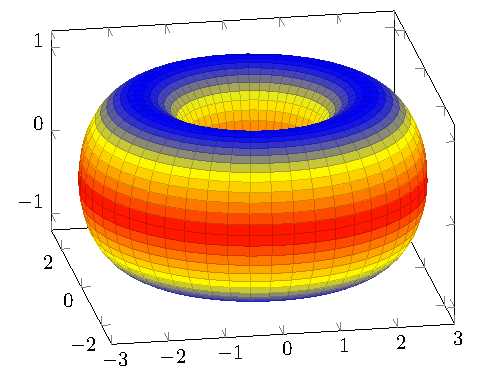
\includegraphics[scale=0.8]{images/c9.2.pdf}
        \caption{Тор.}
        \label{fig:thorus}
    \end{subfigure}
    \hfill
    \begin{subfigure}[b]{0.48\textwidth}
        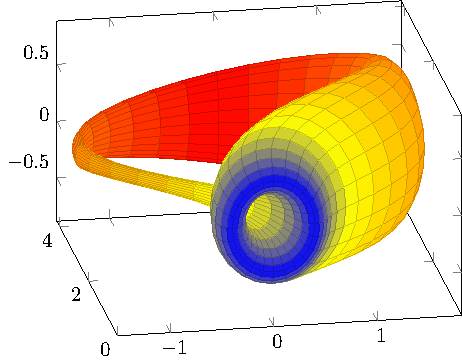
\includegraphics[scale=0.8]{images/c9.1.pdf}
        \caption{Бутылка Клейна.}
        \label{fig:kleyn}
    \end{subfigure}
    \hfill
    \begin{subfigure}[b]{0.48\textwidth}
        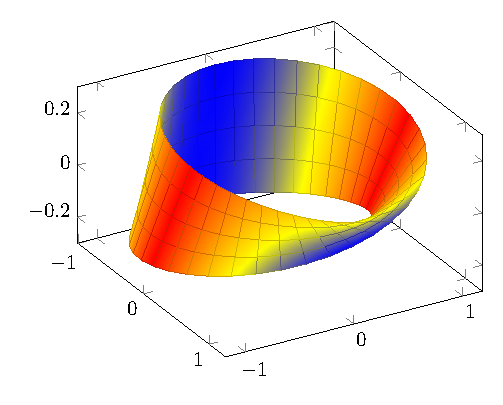
\includegraphics[scale=0.8]{images/c9.3.pdf}
        \caption{Лента Мёбиуса.}
        \label{fig:mobius}
    \end{subfigure}
    \caption{Примеры двумерных многообразий.}
    \label{fig:trio}
\end{figure}

% \begin{figure}[htbp]
%     \centering
%     \subcaptionbox{heading}{content}{heading}
% \end{figure}

\begin{figure}[htbp]
    \centering
    \incfig{c9.5}
    \caption{Склейка тора.}
    \label{fig:c9.5}
\end{figure}

\begin{figure}[htbp]
    \centering
    \incfig{c9.6}
    \caption{Склейка сферы, бутылки Клейна и проективной плоскости (слева направо).}
    \label{fig:c9.6}
\end{figure}

Существует способ описания двумерных многообразий с помощью склейки каких-то кусочков плоскости, как на рисунках \ref{fig:c9.5} и \ref{fig:c9.6}.

Некоторые замечания по поводу проективной плоскости. Рассмотрим модель проективной плоскости. Из курса аналитической геометрии мы знаем, что точками на проективной плоскости можно называть все прямые в $\R^3$, проходящие через начало координат. Тогда рассмотрим сферу произвольного радиуса с центром в начале координат и отождествим точки пересечения с одной прямой. Скажем, что проективная плоскость — это множество пар диаметрально противоположных точек на сфере. Сфера, у которой отождествили противоположные точки — это то же самое, что и полусфера, у которой отождествлены диаметрально противоположные точки на границе. Но с топологической точки зрения такая полусфера и двумерный диск, у которого отождествлены точки на границе — это одно и то же. Склейка противоположных точек на границе диска соответствует склейке квадрата (см.рис.\ref{fig:c9.6}).

%Вроде всё, кроме девятой лекции (от 03.04.2025), здесь теперь расписано полностью. Когда доделаю лекцию, которая была в четверг — пока неясно, но выше есть хотя бы два определения оттуда. Всё, что сегодня (06.04.2025) было дописано, даже не перечитывалось, будьте осторожны!

